\documentclass[dvipdfmx,14pt]{beamer}
\usepackage{float}
\usepackage{pxjahyper}
\usepackage{minijs,amsmath,comment}
\renewcommand{\kanjifamilydefault}{\gtdefault}
\usetheme{Antibes}
\setbeamertemplate{navigation symbols}{}
\setbeamertemplate{footline}[page number]

\title{所得格差の検定と検出力分析}
\author{奥城健太郎 明治大学数学科4年 宮部研究室}
\institute{解析系卒業論文中間発表会}
\date{2017年11月1日(水)}

\begin{document}

\begin{frame}
\frametitle{}
\titlepage
\end{frame}

\begin{frame}
\frametitle{目次}
\large
\begin{itemize}
 \item 所得格差と所得分布
 \item 仮説検定と検出力
 \item 研究内容
 \item 今後の予定
\end{itemize}
\end{frame}

\begin{frame}
\frametitle{所得格差と所得分布}
\ \\ 
所得格差を示す指標に\textcolor{red}{ジニ係数(Gini coefficient)}があり,所得格差が大きいほどジニ係数が大きい \\
\ \\
世界各国のジニ係数 (2014年) \\
{\small
\begin{center}
\begin{tabular}{|c|c|} \hline
 南アフリカ & 0.62 \\ \hline
 中国 & 0.56 \\ \hline
 アメリカ & 0.39 \\ \hline
 日本 & 0.33 \\ \hline
 フィンランド & 0.26 \\ \hline
\end{tabular}
\end{center}
}
\begin{flushright}
\footnotesize https://www.globalnote.jp/post-12038.html
\end{flushright}
\end{frame}

\begin{frame}
\ \\
下図の色のついた部分の面積をAとすると, \\
ジニ係数は2Aで表される
\begin{figure}
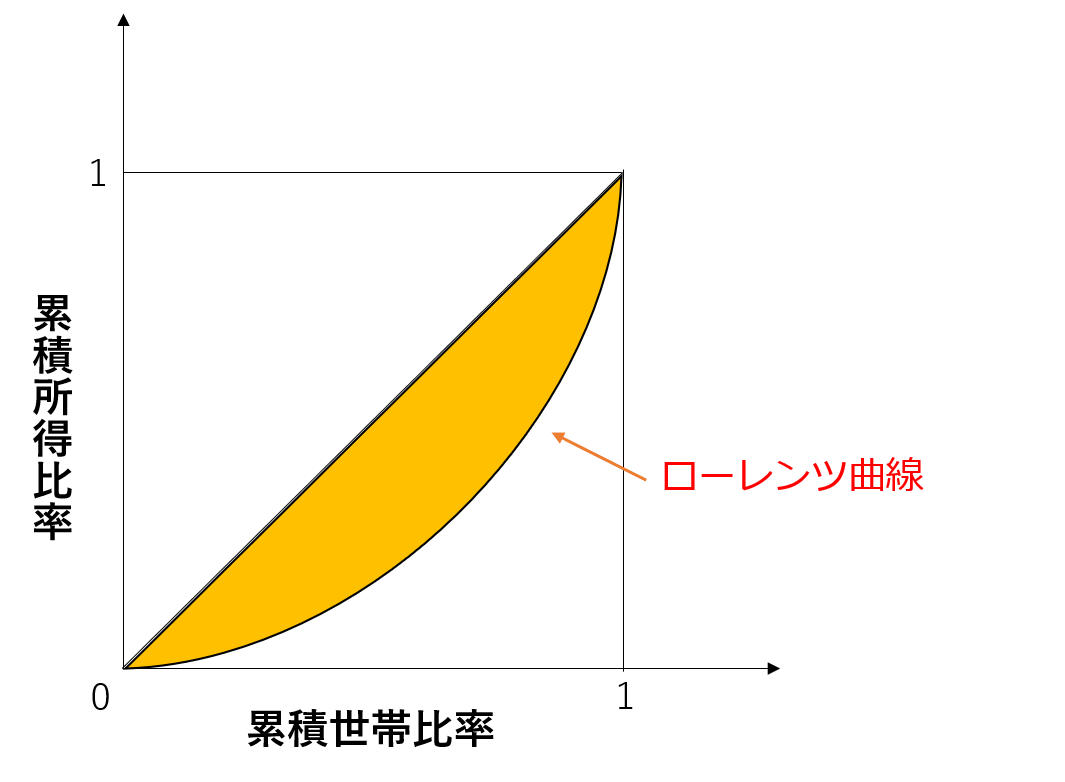
\includegraphics[width=7cm]{図1}
\end{figure}
\end{frame}

\begin{frame}
\ \\
所得の分布は\textcolor{red}{対数正規分布}で表せる \\
(確率変数$X$が対数正規分布$ \Lambda (\mu ,\sigma^2 ) $に従うとき,確率変数$ Y=\log X$は正規分布$ N(\mu ,\sigma^2 )$に従う)
\begin{figure}
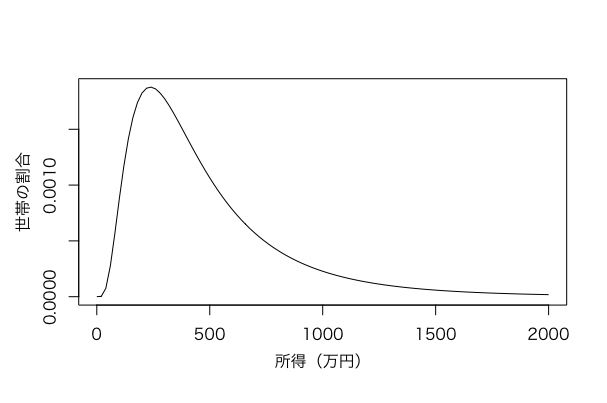
\includegraphics[width=7cm]{curve1}
\end{figure}
\end{frame}

\begin{frame}
実は...
\begin{itemize}
\item ジニ係数は対数正規分布のパラメータ$ \sigma $のみに依存する
\item $ \sigma $が大きいほどジニ係数は大きくなる
\end{itemize}
\ \\ \ \\
\large ジニ係数が与えられたとき,それらが真に違うものと言えるのかを検定したい
\end{frame}

\begin{frame}
\frametitle{仮説検定と検出力}
{\Large ~仮説検定~}
\begin{enumerate}
 \item 中心となる常識的な仮説(\textcolor{red}{帰無仮説})とそれに相対する仮説(\textcolor{red}{対立仮説})を用意する
 \item 検証したい事象に対して,帰無仮説が正しいとした時にその事象またはそれより起こりにくい事象が起こる確率(\textcolor{red}{p値})を求める
 \item p値がある一定の値(\textcolor{red}{有意水準})より大きければ帰無仮説を採択,小さければ帰無仮説を棄却して対立仮説を採択する
\end{enumerate}
\end{frame}

\begin{frame}
\frametitle{}
{\Large ~検出力~}
\begin{itemize}
 \item 帰無仮説が正しいのに帰無仮説を棄却してしまうことを\textcolor{red}{第1種の誤り}という
 \item 帰無仮説が誤っているのに帰無仮説を採択してしまうことを\textcolor{red}{第2種の誤り}という
 \item 第1種の誤りが起こる確率を$ \alpha $ ,第2種の誤りが起こる確率を $ \beta $ という
 \item $ 1-\beta $ を検出力という
\end{itemize}
\end{frame}

\begin{frame}
帰無仮説に対して...
\begin{center}
\begin{tabular}{|c|c|c|} \hline
 & 採択 & 棄却 \\ \hline
 正しい & $ 1-\alpha $ & $ \alpha $ \\ \hline
 誤っている & $ \beta $ & $ 1-\beta $ \\ \hline
\end{tabular}
\end{center}
$ \alpha $を小さくすると$ \beta $は大きくなる \\
そこで,$ \alpha $を一定に保った上で$ \beta $を小さくすることを考える
\end{frame}

\begin{frame}
$ \beta $を小さくするには...
\begin{itemize}
 \item サンプル数を大きくする
 \item 帰無仮説と対立仮説の差を大きくする
\end{itemize}
\ \\ \ \\
サンプル数や仮説間の差を変化させて検出力$ 1-\beta $がどのように変化するかを調べるのが\textcolor{red}{検出力分析}である
\end{frame}

\begin{frame}
\frametitle{研究内容}
\begin{itemize}
 \item 正規分布の分散の比について検定を行うF検定を利用してジニ係数の違いの検定を行う
 \item F検定における検出力をジニ係数を用いて表す
 \item サンプル数によってどのように検出力が変化するのかを調べたい
 \item 検定のシミュレーションも行いたい
\end{itemize}
\end{frame}

\begin{frame}
\frametitle{}
{\large ~分かっていること~}
\\ \ \\
\begin{itemize}
 \item ジニ係数が対数正規分布のパラメータ$\sigma $で表せる
 \item ジニ係数は$\sigma $の定数倍に近い
\end{itemize}
\end{frame}

\begin{frame}
\frametitle{今後の予定}
\begin{itemize}
 \item サンプル数によってどのように検出力が変化するのかを調べる
 \item 検定のシミュレーションを行う
\end{itemize}
\end{frame}

\begin{frame}
\frametitle{参考文献}
\small
\begin{itemize}
 \item 奥村晴彦 『Rで楽しむ統計』 (共立出版,2016)
 \item 稲垣宣生 『数理統計学』 (裳華房,1990)
 \item 永田靖 『サンプルサイズの決め方』 (朝倉書店,2003)
 \item 下方拓 『格差分布の統計的ダイナミクス』 (世界平和研究所,2008)
\end{itemize}
\end{frame}

\begin{frame}
\begin{center}
\Large ご清聴ありがとう \\ ございました
\end{center}
\end{frame}

\end{document}